\chapter{Brief introduction to \LaTeX\ }
\label{assignment:01} 

\begin{flushright}
	\parbox{8cm}
		{
		\begin{flushright}%\color[RGB]{75,0,130} %indigo
		\rule{8cm}{0.75pt}\\
		\vspace*{5mm}
		%\sffamily 
		\begin{itemize}\color[RGB]{0,128,128}
		\item basics of \LaTeX\ as a typesetting language 
		\item \LaTeX\ resources and links
		\item how to include python code in a \LaTeX\ document
		\end{itemize}
		\vspace*{5mm}
		\rule{8cm}{0.75pt}
		\end{flushright}
		}
\end{flushright}

\section{Basic idea of \LaTeX\ }\label{sec:basic}
\LaTeX\ is not a word processor like Microsoft Office, LibreOffice, or Apple's Pages, which are all WYSIWYG (What You See Is What You Get) word processors where the editing window and the output are one and the same. Rather, when you use \LaTeX\, you use a \textit{text editor} (not a word processor) to create the content and the \textit{instructions} for what to do with the content, and then you invoke \LaTeX\ to process this text/instruction file into a printable output. This processing happens quite quickly, and produces a pdf file which can then be viewed on screen and will look exactly as it will print. Since this portable document format is pretty ubiquitous, almost anyone or any device (even smart phones and tablets) can read and display the file. 


To become an expert at \LaTeX\ is a lifelong task; I've been using it for almost 30 years and still do not know all the features available. So don't worry about figuring it all out in a single semester---you only need to know enough to get by, which fortunately, is not so hard. \LaTeX\ is also extensible by numerous packages that allow one to easily add functionality, so there's no limit to what you can do.\footnote{In my course, I provide students with a suitable template file for creating their simulation reports; the goal is to introduce the use of \LaTeX\ as a tool, not make it the \textit{focus} of the course.}

Of course, where \LaTeX\ really shines is in its ability to typeset mathematics in an elegant and efficient manner. You'll even see that the iPython Notebook includes the ability to typeset mathematics---and it uses \LaTeX\ to do so. Thus, by introducing you to \LaTeX\ , you'll be learning a tool that almost all mathematicians and physicists use, and has the depth to serve your writing needs for the rest of your life. \LaTeX\ produces beautifully formatted output that is without peer, so let's get started with a basic introduction.


\section{A simple \LaTeX\ document}\label{sec:simple}
The basic \LaTeX\ text-editor created document consists of a \textit{preamble} and the \textit{Body}. The preamble defines the type of document you want to create---for example: article, letter, report, presentation---and the body is the content. Here is the most simple bare bones \LaTeX\ document possible:\\
\begin{lstlisting}[style=myLaTeXStyle, firstnumber=1]
\documentclass[12pt]{article}
% preamble
\begin{document} % body
Hello World! % this is the standard first program for any language
\end{document}
\end{lstlisting}

The \verb! \documentclass[12pt]{article} !command sets up the document as an article in 12pt type. There are many other document types, some of which are listed in Table~\ref{tab:docTypes}.
\begin{table}
\caption{Some popular \LaTeX\ document types for the documentclass declaration.}
\label{tab:docTypes}
\vspace*{3mm}
\begin{tabular}{ll}
\toprule
Document Type			& description\\
\midrule
article &	for journal articles, short reports, program documentation, etc.\\
report	& for longer reports containing several chapters, small books, thesis.\\
book	& for real books\\
slides &for slides. The class uses big sans serif letters.\\
letter & for writing letters.\\
beamer &for writing presentations (i.e. powerpoint/keynote replacement)\\
\bottomrule
\vspace*{4mm}
\end{tabular}
\end{table}
The preamble may also contain other formatting commands dealing with headers, footers, margins, and even loading other \LaTeX\ packages, and setting up custom commands, but at minimum, you have to have the \verb!\documentclass! command; if you want more information about the options for this command, see \href{http://en.wikibooks.org/wiki/LaTeX/Basics}{http://en.wikibooks.org/wiki/LaTeX/Basics}.

The rest of your document is bounded by the 
\begin{verbatim}
\begin{document}

\end{document}	
\end{verbatim}	
environment, and this is where you put all of your content. Here's a short example of a complete
\LaTeX\ file (on the left), and it's output after typesetting; notice that in order to boldface some text, 
you have to invoke a command:\\[0.5cm]

\begin{adjustwidth}{-.5cm}{.55\textwidth}
\hspace*{.5cm}\textbf{\underline{.tex file:}}\\
\begin{verbatim}
\begin{document}
Here is where you put some
text. To create a new 
paragraph, simply put in a 
blank line, and \LaTeX\ takes
care of the rest.

If you want to make text 
boldface, then you 
use \textbf{this command}.	
\end{document}	
\end{verbatim}	
\end{adjustwidth}
\vspace*{-5.7cm}
\begin{adjustwidth}{.55\textwidth}{0cm}
\textbf{\underline{\LaTeX\ output:}}\\[1cm]
Here is where you put some text. To create a new paragraph, 
simply put in a blank line, and \LaTeX\ takes
care of the rest.

If you want to make text boldface, then you 
use \textbf{this command}.	
\end{adjustwidth}
\vspace*{1in}


Notice that when you are entering straight text, then you do not need to worry about the length of the lines, as \LaTeX\ will format the page for you. You just worry about the content. To create a new paragraph, just put in a blank line; there's no need to indent, for that will also be taken care of when you typeset the document. 

\LaTeX\ also contains specialized environments for making bulleted lists, enumerated lists, captioned figures, footnoting, and anything you can conceivable desire to do. For the most part, \LaTeX\ commands are relatively straightforward, and you'll typically learn environments on a need-to-know basis; nonetheless, it's useful to get an overview of some of the features of \LaTeX\ by reading some of the references that appear on
\href{http://www.latex-project.org/guides/}{http://www.latex-project.org/guides/}---I recommend in particular the three sites listed in Table~\ref{tab:latexRefs}.\\

\begin{table}
\centering
\begin{tabular}{l}\\ \hline
\noindent The (not so) short introduction to \LaTeX\ 2$\mathcal{E}$ at\\ \href{http://ctan.tug.org/tex-archive/info/lshort/english/lshort.pdf}{http://ctan.tug.org/tex-archive/info/lshort/english/lshort.pdf}, \\[1mm]
Getting to grips with \LaTeX\ at\\ \href{http://www.andy-roberts.net/writing/latex}{http://www.andy-roberts.net/writing/latex} and,\\[1mm]
as a general reference online, the WikiBooks \LaTeX\ site at\\ \href{http://en.wikibooks.org/wiki/LaTeX/}{http://en.wikibooks.org/wiki/LaTeX/}.\\
\hline
\end{tabular}
\caption[Several good \LaTeX\ references.]{Several good \LaTeX\ references.}
\label{tab:latexRefs}
\end{table}
%%
\section{\LaTeX\ editor recommendations}
\subsection{\LaTeX\ only editors}
If you are running Linux (or, for that matter Windows, or OS X)
there is a cross-platform open source editor called TeXworks \href{http://www.tug.org/texworks/}{http://www.tug.org/texworks/} that is quite good at writing \LaTeX\ documents, and is what I'd urge you use at the outset. 

On the Mac, the program TeXShop \href{http://pages.uoregon.edu/koch/texshop/}{http://pages.uoregon.edu/koch/texshop/} is singlehandedly responsible for the resurgence of \LaTeX\ on this platform---this open-source editor replaced an extremely expensive commercial alternative, and there was no program like it on Linux or Windows. The TeXworks program was spawned in order to make a cross-platform version of TeXShop. In any case, if you're on the Mac, both of these programs come with the MacTeX distribution which is available at \href{http://www.tug.org/mactex/}{http://www.tug.org/mactex/}.
\subsection{\LaTeX\ and Python editors}
When you are writing a document which includes \LaTeX\ and  python code, it's useful to be able to work on both things within one unified environment. Here are my recommendations for Linux and MacOS. 

For Linux, after much agonizing testing, and looking for something that works pretty much out of the box, I recommend the program GEANY (get it through the Synaptic Package Manager)---make sure to download all the extensions too. When it is installed, you'll want to enable all the plugins. gEdit is also a good program, but I could not get it to correctly compile this document properly, whereas GEANY worked perfectly. 

For Mac OS X, I recommend TextMate, which is the editor I used to compose this text. With TextMate, I could see a file directory of all the \LaTeX\ chapters, python code, and process the \LaTeX\ files and run the python code independently. This is by far the best all-purpose editor for this purpose on the Mac platform.\footnote{VIM and Emacs users would beg to differ!} 
and all my development work for this course is done in this editor which you can get at \href{http://macromates.com/}{http://macromates.com/}.\\
\\
%%
%% Exercise
%%
\rule{\textwidth}{1pt}
\begin{exercise}\label{exer:latex1}	
Open up a \LaTeX\ aware editor, create a simple LaTeX document with a few lines of text, save the file,\footnote{One oddity with \LaTeX\ is that you cannot have a filename with a space in it; instead use a dash or an underscore if you must.}, and typeset it. 
You should get a nice output with the text you typed, and a page number 1 at the bottom of the page. 
There's nothing to hand in here, this is just a test to make sure your \LaTeX\ installation is working. You might start with the ``Hello World!'' example in section~\ref{sec:simple}. 
\end{exercise}
\rule{\textwidth}{1pt}
%%
%%
%%
\section{How to include mathematics into \LaTeX\ }\label{sec:math}
Incorporating mathematical equations in a document is reason enough to use \LaTeX\ over \textit{any} other authoring program. It's notation is simple, powerful, and results is gorgeous typeset equations. There are several ways to include mathematics. 
\subsection{Inline equations}
An inline equation is an equation that occurs right in the course of the text; for instance, if I had a sudden urge to write $\sin \pi = 0$, it's easy to do in \LaTeX;\ all I have to do is type \verb! $\sin \pi = 0$ ! and it will be typeset right in place. Inline equations are typeset in math mode and are demarcated by a beginning and ending dollar sign (therefore, should you actually need a dollar sign symbol to discuss money, you have to use \verb! \$ !).

Inline equations work okay for simple quations, but something more complicated like  $\int_0^{T_0} x^2\;dx = \frac{T_0^3}{3}$ doesn't look so good as an inline equatiuon. For this, we want to use the \verb! \displaymath! environment.

\subsection{Centered and un-numbered equations}
Suppose we want the previous equation to look more readable, but didn't care to number it; then we use two dollar signs and write
\begin{verbatim}
	$$\int_0^{T_0} x^2\;dx = \frac{T_0^3}{3}.$$
\end{verbatim}
which gives us a nicer looking result centered on its own line (in \LaTeX\ parlance, this is called the \verb! \displaymath! environment):
	$$\int_0^{T_0} x^2\;dx = \frac{T_0^3}{3}.$$
Notice that this equation ended a sentence, so I put a period at the end of the equation. Punctuation is important!
There is an equivalent way to get the above equation, which is to use 
\begin{verbatim}
	\[ \int_0^{T_0} x^2\;dx = \frac{T_0^3}{3}.\]
\end{verbatim}
\subsection{Subscripts \& superscripts}
A note about subscripts and superscripts: notice that the lower limit of the definite integral was preceded by an underscore character, and the superscript with an up-caret. For a single character sub or superscript, it is sufficient to use the character immediately after the underscore or up-caret; however, if there is more than one character (like $T_0$), then the sub or superscript must be enlosed by braces.

\subsection{Numbered equations}
If you have a formula that you want to be able to refer back to in the text, then you want to number it (\LaTeX\ will do this automatically for you) and give it a label so that you can refer back to it. For instance, suppose I want to refer to Equation~\ref{eq:sillyIntegral}:
\begin{equation}\label{eq:sillyIntegral}
	\int_0^{T_0} x^2\;dx = \frac{T_0^3}{3}.
\end{equation}
Here is what I typed:
\begin{verbatim}
...suppose I want to refer to Equation~\ref{eq:sillyIntegral}:
	\begin{equation}\label{eq:sillyIntegral}
		\int_0^{T_0} x^2\;dx = \frac{T_0^3}{3}.
	\end{equation}
\end{verbatim}
Use the \verb! \begin{equation} ... \end{equation}! to enter math mode and this tells \LaTeX\ that I want to number the equation. I then gave the equation a descriptive label. I've evolved a strategy to always use a label format that indicates what the item is---i.e. \verb! eq:! for equations, \verb! fig:! for figure labels, etc. You are free to just use \verb! sillyIntegral! if you like. Then to refer to this equation, I type \verb!Equation~\ref{eq:sillyIntegral}! and \LaTeX\  \textit{automatically} takes care of the numbering for me. 
	
\section{How to include Python code in your \LaTeX\ document}\label{sec:listings}

Now, suppose you want to include some Python code (or for that matter, code in practically any computer language) in your report. A nice way to do this is to use the \verb!listings! package (see the WikiBooks site at \href{http://en.wikibooks.org/wiki/LaTeX/Packages/Listings}{http://en.wikibooks.org/wiki/LaTeX/Packages/Listings}). 

\subsection{Short code snippet}
If you have a short \textit{python} code section or \textit{snippet}, your \textit{entire} \LaTeX\ code might look like this:
\begin{lstlisting}[label=includePythonSnippet, caption =Including a short python snippet,style=myLaTeXStyle, firstnumber=1]
\documentclass[12pt]{article}
\usepackage{listings} % loads the listings package
\usepackage[usenames,dvipsnames]{color} % load a color package
% define some colors
\definecolor{light-gray}{gray}{0.97} 
\definecolor{lightGreenPython}{RGB}{240,255,240}
\definecolor{wheat}{RGB}{252,247,234}
%
%%% The following command defines some options in the listings
%%% package to nicely format python code; feel free to use it.

%%%
\lstdefinestyle{pythonSnippet}{
language=python, 
backgroundcolor=\color{wheat}, 
frame=leftline, 
framerule=0.5pt, 
rulecolor=\color{RoyalPurple}
}

%%%
\begin{document}
%
\noindent Here is a code snippet:
\begin{lstlisting}[style = pythonSnippet]
y0, v0, t = 10.0, 0.0, 2.0    # defines the variables 
y = y0 + v0 * t -4.9 * t**2   # computes the y position 
print y                       # prints out the value of y 
\end\{lstlisting} 
\end{document}
\end{lstlisting}


You can see the output produced by running this file through the \LaTeX\ engine in here:\footnote{Note that due to the difficulty of having Listing~\ref{includePythonSnippet} include an example of the \textit{listings} package within the \textit{listings} environment there was an unavoidable backslash in line 29 before lstlisting which you should remove in an actual \LaTeX\ file. }
\begin{lstlisting}[style=pythonSnippet]
y0, v0, t = 10.0, 0.0, 2.0    # defines the variables 
y = y0 + v0 * t -4.9 * t**2   # computes the y position 
print y                       # prints out the value of y 
\end{lstlisting} 

\subsection{Extended Section of Code}
If you have an entire python script, it's much more convenient to \textbf{not} have to cut and paste your code into the \LaTeX\ file since it's often the case that you find a small error in your code and then you need to re-paste the code or edit it directly in the \LaTeX\ file itself. A much nicer way to do this is to use the ability of the \verb!listings! package to directly include the file containing the python code. What follows is the complete \LaTeX\ code that will allow you to accomplish this. \\[5mm]

\begin{lstlisting}[style=myLaTeXStyle, firstnumber=1]
\documentclass[12pt]{article}
\usepackage{listings} % loads the listings package
\usepackage[usenames,dvipsnames]{color} % load a color package
% define some colors
\definecolor{light-gray}{gray}{0.97} 
\definecolor{lightGreenPython}{RGB}{240,255,240}
\definecolor{wheat}{RGB}{252,247,234}
%
%%% The following command defines some options in the listings
%%% package to nicely format python code; feel free to use it.

%%%
\lstdefinestyle{pythonSnippet}{
language=python, 
backgroundcolor=\color{wheat}, 
frame=leftline, 
framerule=0.5pt, 
rulecolor=\color{RoyalPurple}
}
\lstdefinestyle{MyPythonStyle}{
language=python, 
frame=lines, 
framerule=0.5pt, 
rulecolor=\color{RoyalPurple}, 
numbers=left, 
stepnumber=2, 
numberstyle=\tiny, 
numbersep=5pt
}
\begin{document}	
\lstinputlisting[label=plot, 
caption=\LaTeX\ output by direct reference to a python file.
]
{Code/Assignment_01/plot.py}
\end{document}
\end{lstlisting}

The above \LaTeX\ code produces the output shown in (Listing~\ref{plot}). Notice that the python file is well commented---a habit you should get into. Good code is well-documented, and easily understood by anyone familiar with the language. \\

\lstinputlisting[label=plot, caption=\LaTeX\ output by direct reference to a python file.]
{Code/Assignment_01/plot.py}


Now you can see the advantage of this method, right? You can work on the \LaTeX\ code for your report, and at the same time, you can be working on the python code and the \textit{Listings} package takes care of including the final version of the code automatically since it merely links to this file and then formats the text file nicely including syntax highlighting. Good luck trying to do that seamlessly in any other word processor!

Also notice that at the beginning of the python file, I placed a description of the python script within triple quotes. This is the format python uses for documentation strings. This triple-quoted string provides a good description of what the python code does, and can be accessed interactively from a python interpretter, as we will see soon. As always, you can read more about this by performing a web search for ``Python docstrings''. 

\section{Final Words on \LaTeX\ }
\LaTeX\ is a huge package and it takes years to learn. That's both good news and bad. The bad, of course, is that it takes some getting used to using, and when you make an error, the feedback that \LaTeX\ gives you is not always transparent. 

On the other hand, when you do get an error, a little googling of the error message will often set you straight. And, you likely have a few experts on \LaTeX\ in your friendly neighborhood physics or mathematics departments that can help you. In addition, there is lots of room to grow in \LaTeX\ ; you can design entire books, all typeset in gorgeous manner. 

A good idea at this point is to sit down with a good \LaTeX\ tutorial and practice your new \LaTeX\ skills with the following exercises.

\rule{\textwidth}{1pt}
\begin{exercise}\label{ex:latexStep1}
When you create a \LaTeX\ document, it should have the extension .tex, and after you typeset it, several other files will appear (depending on the document); thus it's useful to keep a \LaTeX\ document in its own folder. Go through the following steps, designed to get you in a good organizational file management habit.
\captionsetup[table,figure]{list=no}
\begin{enumerate}
	\item Create a folder called \texttt{ComputationalPhysics} (no spaces) and inside that, create a folder called \texttt{LaTeXPractice} and with that, a new \LaTeX\ document whose \texttt{documentclass} is \texttt{article} and is called	\texttt{exercise1.tex}. You may use any \LaTeX\ editor you like, but for simplicity, I recommend that you use \texttt{Texworks} as it is available on all three major computing platforms. You can create this file from the \texttt{File > New from Template} menu option, and choose the \texttt{article} document class. Add the following to your document:
	\item Add title, author, and date information, and make a title appear at the top of the page. 
	\item Add a paragraph or two, and include some \textbf{boldface text}, some \textit{italic text}, and the famous equation 
	$E = m c^2$, both as an inline formula and as a formula on it's own line like this:\\
	$$ E = m c^2. $$
	\item Add an enumerated list.
	\item Add a two column \texttt{Table} like this:
	\begin{table}\centering
		\begin{tabular}{c l}\\ \hline
			Category & Favorite thing\\ \hline
			food & \\
			song & \\
			exercise & \\ \hline
		\end{tabular} 
	\caption{Some of my favorite things.}
	\end{table}
    Fill in the second column.
	\item Download a full resolution picture of Albert Einstein from \textit{Wikipedia}, place it in a \texttt{Figures} folder within the \texttt{LaTeXPractice} folder. Display the .jpg figure in your paper using the \LaTeX\ \texttt{figure} environment as shown in Figure~\ref{fig:Einstein}. Make the image 6 cm wide. Notice that \LaTeX\ puts the image wherever it pleases. Don't worry about that right now. 
	\begin{figure}
		\centering
		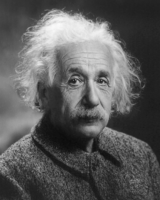
\includegraphics[width=6cm]{Figures/introToLatex/Einstein}
		\caption{Albert Einstein, image in the public domain; from \textit{Wikipedia}.}
		\label{fig:Einstein}
	\end{figure}	
	\item when you are done, submit your work electronically accoring to the instructions in Appendix~\ref{app:submission}. Of course, in this case, you will not have a \texttt{Code, Data,} or \texttt{References} folder.
\end{enumerate}
\captionsetup[table,figure]{list=yes}
\end{exercise}
\rule{\textwidth}{1pt}
	
